\chapter{概述}
\pagenumbering{arabic}

本课程主要讨论用如何计算机模拟随机事件,以及以此为基础的优化算法、数值方
法和数学模型。随机,或者说不确定性,是我们所处世界的一个基本属性。而我
们人类,特别是受到过严格科学训练的人,其思维结构往往是偏向确定性的。这
就导致一部分人,甚至是受过高等数学教育的人,在对不确定性事物的直观理解
上,会有偏差。最常见的,比如赌徒心理:一个骰子如果已经连开十四次大,那
么它下一次开小的概率会不会上升?这个问题相对简单一点,我们来看一个更复
杂的游戏。

\section{例子:羊还是车 —— 对概率论结果的数值验证}
这个游戏最早来源于一个北美的电视节目,有点像综艺节目
\cite{Blues2016Edos}。最终环节主持人要来宾挑选礼物。礼物藏在三扇门后面,
两个门后面是一只山羊,而一扇门后面是一辆汽车。来宾知道礼物是什么,但不
清楚哪扇门后面是汽车。他只能随机打开一扇门,得到他的奖品。显然,汽车价
值要远高于山羊,所以来宾都更想得到汽车。主持人是知道哪扇门后是汽车的。
在来宾挑选了一扇门,尚未打开的时候,主持人会打开一扇藏了山羊的门(注意
  他总能做到这一点)。此时,来宾有一个选择,是坚持自己的门,还是换一扇?

\begin{figure}[!ht]
\centering
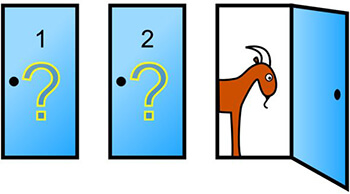
\includegraphics[width=0.7\textwidth]{images/game.jpg}
\caption{车还是羊?}
\label{fig::game}
\end{figure}

这个场景在电影《决胜21点》中也有出现。剧中男主角用概率论分析了这个问题:
``如果不换,那么选中车的概率就一直保持最初的$1/3$;而在主持人打开门以
后换一扇门,同时又能选中车的概率则是$2/3$。''我们知道好莱坞电影里的数学
理论大多数不那么严肃。那么这个主角也是在胡扯么?

选修了这门课的同学都不难自己用概率论验证,主角是正确的。但即便是一个严
格的概率论推导过程,真的就能真正说服我们么?是不是有一部分同学(甚至是
  大部分同学),始终觉得这就是在玩弄概率论。直觉上似乎始终有一个声音告
诉我们,一个确定的选择导致的已经发生的概率,不会因后续事件而改变。

对这件事情最好的回答,无过于我们真的去玩这个节目足够多的次数,比如
10000次,然后统计不同策略的得失。(注意是统计,这一点电影还是错了,它
  始终说是上面的分析是一个统计学过程,而事实上应该是概率论。真实的去数
  充分多的游戏中不同策略的结果,才是统计。统计就是数数字,而概率则是测
  度论。)于是我们首先需要10000辆车和20000只羊?如果谁愿意赞助我一定不
会反对。但更实际的,我们考虑一下能否在计算机中模拟这10000次游戏来达到
同样的统计结论。

为方便起见,在这门课中我选择Python 3.0来描述算法和实现程序。理由是这是
一门最接近自然语言和伪代码风格的语言。同时它又是大数据领域被广泛接受的
语言。我们不会专门讲述如何使用Python语言编程。而是在使用的过程中不断熟
悉这门语言。对于从未接触过Python的同学,我们会有一个简单的入门环节。可
能在上机课程或者以讲义的形式提供。

我们直接来读代码,Python的代码非常容易阅读。算法\ref{alg::game}给出了
用计算机模拟整个游戏的过程。并提供了simulation函数用于测试不同的策略,
并分别对两种策略进行了10000次模拟,统计了最终结果。一次典型的结果如下
(注意每次模拟的结果都会不同,如果是真随机的话):

\begin{lstlisting}
win rate of never exchange: 0.3357
win rate of exchange: 0.671
\end{lstlisting}

这个结果清晰地表明在``实际''游戏过程中,换与不换确实会有实质的不同。
概率论的结果并不是一个观点,而是客观事实。相反我们的直观并不一定总是正
确的。特别对于随机事件,我们要更加小心对待。最后让我们回到对概率论结果
的直观理解中。只要考虑一下,如果第一次选错的嘉宾,他在主持人开门之后换
一扇门一定可以得到车。而第一次选错的概率就是$2/3$。通过这个例子,我们
明白计算机模拟确实可以在我们发生怀疑的时候,帮助我们理解一个随机事件的
本质,即便已经有了概率估计,它也可以帮助我们建立正确的直观去理解概率结
果。

在这一过程中,真正起作用的是两件事情,第一是随机数的产生;第二是计
算机能够高效率地产生大量重复试验的结果,并可以对结果进行有效的统计。概
率论在这里确实是一个指导性思想。但我们的具体实现始终都是统计过程。这二
者能够达成一致的基本原理就是大数定律和中心极限定律。概率论是数学,它的
结论是客观事实。但如何理解是一个严重的问题。而统计实现过程也必须足够小
心。比如这个算法\ref{alg::game}大家觉得有没有严重的缺陷使得它至多只
是一个模拟验证,而不能称为是一个数学结论?

问题就在于我们用计算机产生的``随机数''只能是伪随机数。它具备像一个真正
随机序列那样的分布特征,比如这里的随机数是均匀分布的,那么它在均匀性上
会表现的和真正的随机序列``几乎''一样。然而,它事实上是有规律的。这使得
我们一方面需要认真研究如何才能更高质量和高效率地产生伪随机数,另一方面
需要对这件事情有充分的认识,并在设计算法的时候小心谨慎。科研历史上确实
发生过由于伪随机序列的隐含规律导致模拟结果错误的事情。

\begin{minipage}[!ht]{0.8\textwidth}
\vspace{3ex}
\refstepcounter{alg}
\label{alg::game}
\begin{center}
 算法 \arabic{chapter}.\arabic{alg} 游戏:羊还是车
\end{center}
\small
\begin{tabular}{lll}
  \hei 输入&total&模拟的次数\\
  \hei 输出&&显示两种策略的胜率
\end{tabular}
\begin{lstlisting}[style = python, escapechar = \%]
def setup_game():
    # 三扇门初始化成都藏了羊。
    doors = [Prize.goat, Prize.goat, Prize.goat]
    # 先随机挑选一扇门,将羊换成车。
    car = np.random.randint(0, 3)
    doors[car] = Prize.car
    # 嘉宾挑选一扇门,然后主持人打开一扇藏有羊的门。
    guest = np.random.randint(0, 3)
    for host in range(0, 3):
        # 既不是藏有车的门,也不是嘉宾挑选的
        if host is not car and host is not guest:
            break
    return doors, guest, host

# 策略A, 打死也不换。这也是个函数,没毛病。
def strategyA():
    # do nothing.
    return

# 策略B, 换换更健康。
def strategyB(doors, guest, host):
    for new in range(0, 3):
        # 既不是之前挑选的门,也不是主持人打开的
        if new is not guest and new is not host:
            break
    return new

def simulation(total):
    # 嘉宾和主持人的选择,初始为-1。
    win = 0
    for i in range(total):
        doors, guest, host = setup_game()
        strategyA()
        if doors[guest] is Prize.car:
            win = win + 1
    print("win rate of never exchange:", win/total)
    win = 0
    for i in range(total):
        doors, guest,host = setup_game()
        guest = strategyB(doors, guest, host)
        if doors[guest] is Prize.car:
            win = win + 1
    print("win rate of exchange:", win/total)
    return
\end{lstlisting}
\end{minipage}

\section{随机优化算法简介}
除了对一个随机事件进行直接模拟。随机算法还可以用在优化求解上。这一类算
法经常被归入Monte Carlo方法,也有人将其进一步分化成Monte Carlo方法和
Las Vegas方法。它们分别代表了两种侧重略有区别的策略。不太严格地说,对
一个优化问题
\begin{equation}
\min f(x), x \in \mathcal{D}. 
\label{eq::min}
\end{equation}
这里$\mathcal{D} \in \mathbb{R}^m$是问题的定义域, $m$是维数. Monte
Carlo法的思路是在$\mathcal{D}$中以某种分布进行随机采样$\xi \in
\mathcal{D}$, 并根据$f(\xi)$的结果不断调整分布. 然后随着采样次数$n$
的增多,有
$$
\lim_{n \to \infty}E(\xi) \stackrel{1}{\hookrightarrow} x^*.
$$其中$x^*$是问题(\ref{eq::min})的真解。而Las Vegas方法则不停地随机投
点并根据反馈调整分布,直到在某一次测试中,发现$\xi$严格地等于$x^*$才能
结束。显然,Las Vegas方法可以看作是Monte Carlo方法的一个特例。而且它更
加适用于离散优化。我们在之后的讨论中不再区分二者。

Monte Carlo法的实际应用也远比优化要宽广。理论上它几乎可以解决任何问题
(在不计效率的前提下)。下面给一个几乎所有Monte Carlo讲义都会提到的例
子,计算圆面积.

\begin{figure}[!ht]
\centering
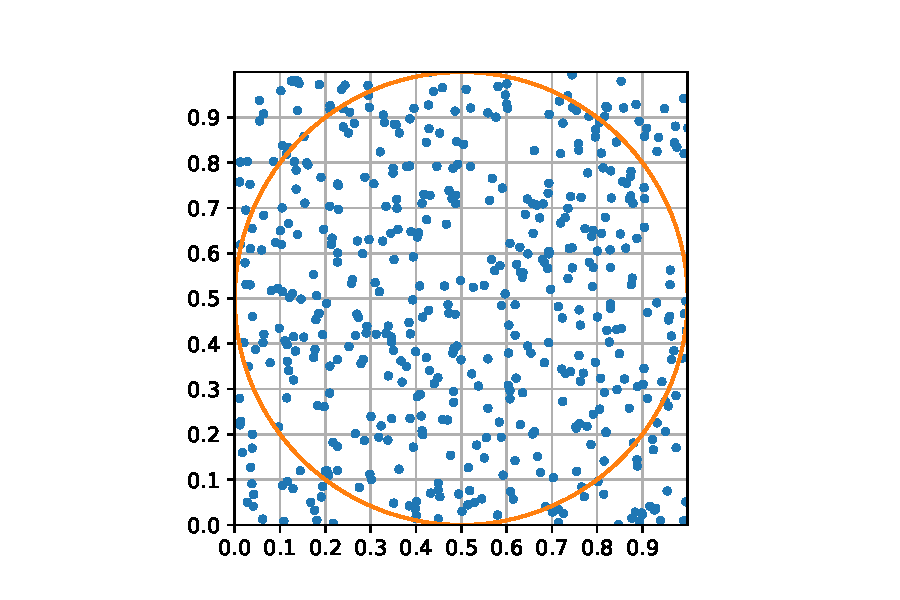
\includegraphics[width=0.7\textwidth]{images/circle.pdf}
\caption{求圆面积}
\label{fig::circle}
\end{figure}

如图\ref{fig::circle},我们通过随机投点来估计这个内接在单位正方形内部
的单位圆的面积。我们要确保每一次投点都是满足在单位正方形内均匀分布的,
这样点落在圆内的概率$p$就是圆面积和正方形面积之比。因此我们只要统计落
在圆内和所有的点的数目,那么它们二者之比就会在大数定律的控制下依概
率收敛到$p$。这样就可以计算出圆面积。我们在今后的学习中会用严格的概率
理论重建这个过程,而现在先用朴素的语言描述以便于直观理解,好在具体的算
法和程序过程仍然是严格的。

\begin{minipage}[!ht]{0.8\textwidth}
\vspace{3ex}
\refstepcounter{alg}
\label{alg::circle}
\begin{center}
 算法 \arabic{chapter}.\arabic{alg} Monte Carlo法求圆面积
\end{center}
\small
\begin{tabular}{lll}
  \hei 输入&times&抽样次数\\
  \hei 输出&&圆面积的计算值
\end{tabular}
\begin{lstlisting}[style = python, escapechar = \%]
def area_circle(times):
    inside = 0
    dots = np.random.rand(2, times)
    for i in range(times):
        x = dots[0, i] - 0.5
        y = dots[1, i] - 0.5
        if x * x + y * y < 0.25:
            inside += 1
    return inside / times
\end{lstlisting}
\end{minipage}

%% 积分的例子,即求
%% \begin{equation}
%%   I = \int_\mathcal{D}f(x) dx, \mathcal{D} \in \mathbb{R}^m.
%% \label{eq::int}
%% \end{equation}
%% 这里如果$f(x) = 1$, 则问题就是求$m$区域$\mathcal{D}$的测度。比如$m =
%% 2$就是求$\mathcal{D}$的面积。我们来看一个特例:
%% \begin{equation}
%%   I = \int_0^1f(x) dx, \mathcal{D} \in \mathbb{R}^m.
%% \end{equation}

由于我们在计算圆面积的时候没有使用圆面积公式。因此实际上我们可以通过这
个程序来估计$\pi$值。这个其实不是我们接触到的第一个求圆周率的随机算法。
大家还记得上概率论时介绍过的浦丰投针实验么?那就是一个相当硬核的物理随
机模拟算法。当然它也能计算机模拟,但是要小心处理边界的情况(针掉到平行
  线组之外去了)。

我们现在来观察我们求得的$\pi$值。和所有随机算法一样,它的结果是不稳定
的。比如图 \ref{fig::variation}中给出了100组独立随机模拟的结果,每次模
拟都是10000个随机投点。可以看到它们在精确的$\pi$值附近波动。

\begin{figure}[!ht]
\centering
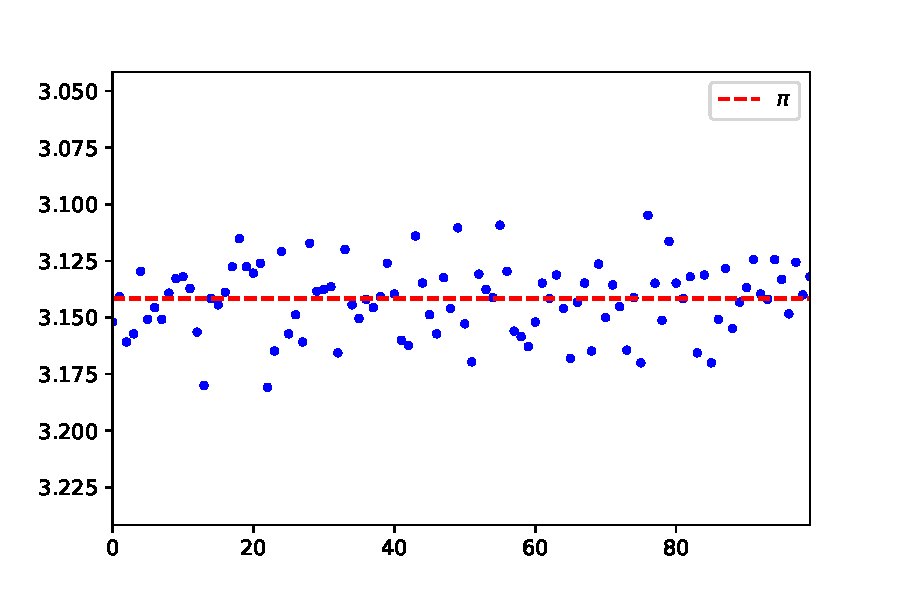
\includegraphics[width=0.7\textwidth]{images/variation.pdf}
\caption{Monte Carlo法求圆周率, 每次10000次随机投点,重复了100组。}
\label{fig::variation}
\end{figure}

增加投点数量显然可以减少模拟结果的波动,或者说,从随机算法的角度,提高
结果的精度。从图 \ref{fig::number2variation}可以看到,随着投点的增加,
模拟结果越来越聚集到精确$\pi$值的附近。这张图也很形象地表现了什么叫依
概率收敛。

\begin{figure}[!ht]
\centering
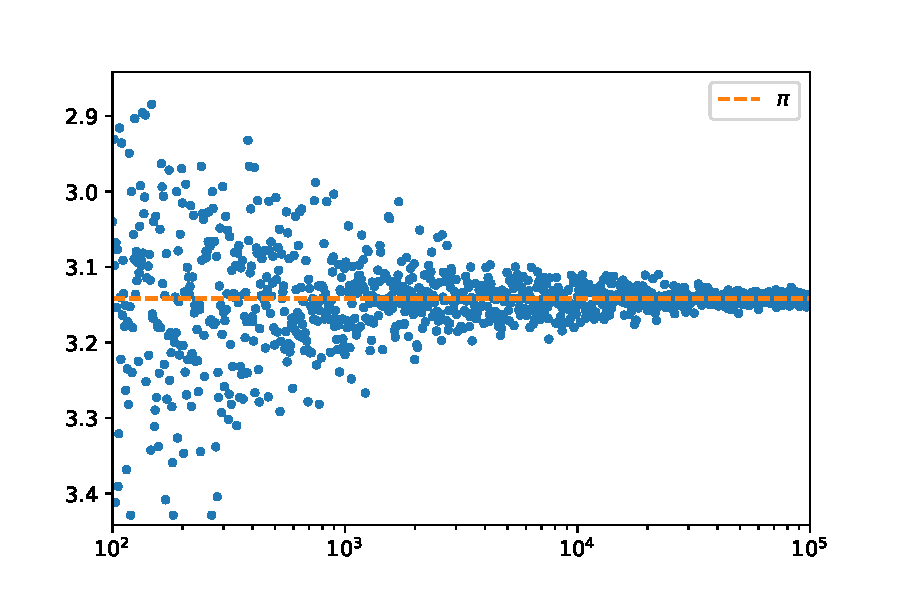
\includegraphics[width=0.7\textwidth]{images/number2variation.pdf}
\caption{Monte Carlo法求圆周率, 投点数从$10^2$到$10^5$, 按$\log$分布
  做了1000组。}
\label{fig::number2variation}
\end{figure}

Monte Carlo方法的优点和缺点都一样明显。好处是它只基于随机投点,整个过
程非常简单机械,非常适合计算机完成。在很多数学上根本无法建模的问题中,
它也能很好地实现。它确实是一种``万能''的方法。坏处就是,我们稍微思考一
下就能明白,它有效完全依赖于大数定律和中心极限定理。即随着独立试验的增
加,均值总是会依概率收敛到(设计好的)期望。那么误差在这里就会收敛到方
差!显然,误差是$\mathrm{O}(1 / \sqrt{n})$的(后续课程我们会精确分析这
  一过程)。这意味这如果我们在十进制下要增加一位有效数字,那么工作量会
增加100倍。而一般的数值积分方法,误差一般都是$\mathrm{O}(1 / n^p), p >
1$阶的。所以只有在相对复杂,经典数值方法无法给出高效算法的情况下,我们
才会考虑Monte Carlo方法。比如,极高维度的数值积分。我们注意到,经典数
值积分方法是维数相关的,随着空间维数的增加,为了得到同样阶精度,积分点
的数量也要以空间指数增加。比如在3维要达到$\mathrm{O}(1 / n^p), p > 1$
的精度,相对1维来说,积分点也要从$n$个增加到$\mathrm{O}(n^3)$个。于是
对于一些超高维数问题,经典数值方法变得非常昂贵。然而,大家也许已经注意
到,Monte Carlo方法是维数无关的,不管这个区域是几维,我们要做的就是随
机投点,数数。当然,实际上产生一个$m$维空间的随机点,相比1维空间,工作
量是其$m$倍。但至少只是一个线性增长。因此维数越高,Monte Carlo方法的优
势越明显。

\section{本课程内容}
在这个学期,我们的重点既不在概率论,也不在统计,甚至也不会专门讲太多的
计算机编程。(当然概率论是一切的理论基础,所以如果你没有学过概率论,那
  么赶紧去自学一下也许还能活。)我们将注意力更多地集中在随机算法和相应
的技术实现上。这其实是一门优化或者数学规划(Operations Research)的分支
课程。它变得如此重要的原因相信大家都是理解的。在目前大数据和AI领域的最
前沿,随机优化算法正在发挥巨大的作用。然而在传统的授课体系中,不论在计
算机学院还是数学院,和随机优化有关的内容之前都不是很受重视,至少缺乏系
统性的讲述。本课程的设计初衷就是试图弥补这个空缺。在接下去的一个学期中,
我们将从随机数的产生和随机抽样开始,逐步讨论Monte Carlo方法、模拟退火
算法、遗传算法等经典的随机优化方法,介绍它们的原理和实现。同时我们也会
重点分析一些比较重要的具体算法,比如神经网络中经常采用的随机梯度下降算
法。此外,我们也会解析几个重要案例,来体会这些理论和技术是如何在具体问题
中得到应用的。

由于这是一门面向全新领域的全新课程,所以以上的一切都还不是定案。在学习
过程中,我们可能随时根据需要增删。同时可能也会有大量的参考材料和技术资
料需要课外阅读。希望通过我们这一学期的努力,能够初步建立起这样一门关键
课程的框架和雏形。在这个过程中,需要我们每一位参与者的共同努力。
